% Options for packages loaded elsewhere
\PassOptionsToPackage{unicode}{hyperref}
\PassOptionsToPackage{hyphens}{url}
\PassOptionsToPackage{dvipsnames,svgnames*,x11names*}{xcolor}
%
\documentclass[
  russian,
  a4paper,
]{article}
\usepackage{lmodern}
\usepackage{setspace}
\setstretch{1.2}
\usepackage{amssymb,amsmath}
\usepackage{ifxetex,ifluatex}
\ifnum 0\ifxetex 1\fi\ifluatex 1\fi=0 % if pdftex
  \typeout{Setting Fonts for pdftex}
  \usepackage[T2A,T1]{fontenc}
  \usepackage[utf8]{inputenc}
  \usepackage{textcomp} % provide euro and other symbols
\else % if luatex or xetex
  \typeout{Setting Fonts for luatex or xetex}
  \usepackage{unicode-math}
  \defaultfontfeatures{Scale=MatchLowercase}
  \setmainfont[]{Times New Roman}
  \setmonofont[
    Contextuals={Alternate} % Activate the calt feature
  ]{Fira Code}
\fi
% Use upquote if available, for straight quotes in verbatim environments
\IfFileExists{upquote.sty}{\usepackage{upquote}}{}
\IfFileExists{microtype.sty}{% use microtype if available
  \usepackage[]{microtype}
  \UseMicrotypeSet[protrusion]{basicmath} % disable protrusion for tt fonts
}{}

\makeatletter
\@ifundefined{KOMAClassName}{% if non-KOMA class
  \IfFileExists{parskip.sty}{%
    \usepackage{parskip}
  }{% else
    \setlength{\parindent}{0pt}
    \setlength{\parskip}{6pt plus 2pt minus 1pt}}
}{% if KOMA class
  \KOMAoptions{parskip=half}}
\makeatother

\usepackage{xcolor}
\IfFileExists{xurl.sty}{\usepackage{xurl}}{} % add URL line breaks if available
\IfFileExists{bookmark.sty}{\usepackage{bookmark}}{\usepackage{hyperref}}
\hypersetup{
  pdftitle={Домашняя работа по Математической Статистике},
  pdfauthor={Митин Арсений (3 курс, СКБ171)},
  pdflang={ru},
  pdfkeywords={Statistics},
  colorlinks=true,
  linkcolor=blue,
  filecolor=Maroon,
  citecolor=Blue,
  urlcolor=Blue,
  pdfcreator={LaTeX via pandoc}}
\urlstyle{same} % disable monospaced font for URLs
\usepackage[margin=2.5cm]{geometry}
% \usepackage{textcomp}
\usepackage{listings}
\newcommand{\passthrough}[1]{#1}
\lstset{defaultdialect=[5.3]Lua}
\lstset{defaultdialect=[x86masm]Assembler}

% https://github.com/tonsky/FiraCode/wiki/LaTeX-instructions
\usepackage[verbatim=true]{lstfiracode} % for FiraCodeStyle
\usepackage{MnSymbol} % for \rhookswarrow
\lstset{
  language          = Haskell,
  backgroundcolor   = \color[HTML]{FFFFFF},
  basicstyle        = \color[HTML]{000000}\ttfamily,
  breaklines        = true,
  breakatwhitespace = true,
  breakautoindent   = true,
  commentstyle      = \color[HTML]{009900},
  frame             = l,
  framesep          = 7pt,
  keepspaces        = true,
  keywordstyle      = \color[HTML]{000099},
  moreliterate      = {*}{{\firaseries*}}1,
  numbers           = left,
  numberstyle       = \small\color[HTML]{808080},%\nocopynumber,
  numbersep         = 10pt,
  prebreak          = \raisebox{0ex}[0ex][0ex]{\ensuremath{\rhookswarrow}},
  postbreak         = \raisebox{0ex}[0ex][0ex]{\ensuremath{\hookrightarrow\space}},
  rulecolor         = \color[HTML]{808080},
  showspaces        = false,
  showstringspaces  = false,
  stringstyle       = \color[HTML]{009966},
  tabsize           = 2,
  upquote           = true,
}

\lstset{style=FiraCodeStyle}


\usepackage[
  symbol=$\uparrow$,
  numberlinked=false,
]{footnotebackref}

\usepackage{graphicx,grffile}
\makeatletter
\def\maxwidth{\ifdim\Gin@nat@width>\linewidth\linewidth\else\Gin@nat@width\fi}
\def\maxheight{\ifdim\Gin@nat@height>\textheight\textheight\else\Gin@nat@height\fi}
\makeatother
% Scale images if necessary, so that they will not overflow the page
% margins by default, and it is still possible to overwrite the defaults
% using explicit options in \includegraphics[width, height, ...]{}
\setkeys{Gin}{width=\maxwidth,height=\maxheight,keepaspectratio}
% Set default figure placement to htbp
\makeatletter
\def\fps@figure{htbp}
\makeatother
\setlength{\emergencystretch}{3em} % prevent overfull lines
\providecommand{\tightlist}{%
  \setlength{\itemsep}{0pt}\setlength{\parskip}{0pt}}
\setcounter{secnumdepth}{2}

% Make \paragraph and \subparagraph free-standing
\ifx\paragraph\undefined\else
  \let\oldparagraph\paragraph
  \renewcommand{\paragraph}[1]{\oldparagraph{#1}\mbox{}}
\fi
\ifx\subparagraph\undefined\else
  \let\oldsubparagraph\subparagraph
  \renewcommand{\subparagraph}[1]{\oldsubparagraph{#1}\mbox{}}
\fi


% Make use of float-package and set default placement for figures to H.
% The option H means 'PUT IT HERE' (as  opposed to the standard h option which means 'You may put it here if you like').
\usepackage{float}
\floatplacement{figure}{H}

\newfontfamily\cyrillicfont{Times New Roman}[Script=Cyrillic]
\definecolor{dodgerblue}{HTML}{1E90FF}
\makeatletter
\@ifpackageloaded{subfig}{}{\usepackage{subfig}}
\@ifpackageloaded{caption}{}{\usepackage{caption}}
\captionsetup[subfloat]{margin=0.5em}
\AtBeginDocument{%
\renewcommand*\figurename{Figure}
\renewcommand*\tablename{Table}
}
\AtBeginDocument{%
\renewcommand*\listfigurename{List of Figures}
\renewcommand*\listtablename{List of Tables}
}
\newcommand*\listoflistings\lstlistoflistings
\AtBeginDocument{%
\renewcommand*{\lstlistlistingname}{List of Listings}
}
\makeatother
\ifnum 0\ifxetex 1\fi\ifluatex 1\fi=0 % if pdftex
  \typeout{Setting Languages for pdftex}
  \usepackage[shorthands=off,main=russian]{babel}
\else % if luatex or xetex
  \typeout{Setting Languages for luatex or xetex}
  \usepackage{polyglossia}
  
  % See issue https://github.com/reutenauer/polyglossia/issues/127
%   \renewcommand*\familydefault{\sfdefault}

  \setmainlanguage[]{russian}
%
% When using babel or polyglossia with biblatex, loading csquotes is recommended
% to ensure that quoted texts are typeset according to the rules of your main language.
%
\usepackage{csquotes}
\fi

\title{Домашняя работа по Математической Статистике}
\author{Митин Арсений (3 курс, СКБ171)}
\date{26.10.2019}


\usepackage{fancyhdr}
\pagestyle{fancy}
\fancyhf{}
\fancyhead[LO,LE]{\leftmark}
\fancyhead[RO,RE]{\rightmark}
\fancyfoot[C]{\thepage}
\renewcommand{\headrulewidth}{0.4pt}
\renewcommand{\footrulewidth}{0.4pt}


\begin{document}
\maketitle

\newpage
{
\hypersetup{linkcolor=}
\setcounter{tocdepth}{2}
\tableofcontents
\newpage
}
\providecommand{\mathFunc}[4]{#1\left#2\, #3 \,\right#4}
\providecommand{\mathbbFunc}[4]{\mathFunc{\mathbb{#1}}{#2}{#3}{#4}}
\providecommand{\mathrmFunc}[4]{\mathFunc{\mathrm{#1}}{#2}{#3}{#4}}
\providecommand{\Prob}[1]{\mathbbFunc{P}{(}{#1}{)}}
\providecommand{\Expect}[1]{\mathbbFunc{E}{[}{#1}{]}}
\providecommand{\Var}[1]{\mathrmFunc{Var}{[}{#1}{]}}

\hypertarget{ux437ux430ux434ux430ux43dux438ux435-1}{%
\section{Задание №1}\label{ux437ux430ux434ux430ux43dux438ux435-1}}

\hypertarget{ux432ux44bux431ux43eux440-ux440ux430ux441ux43fux440ux435ux434ux435ux43bux435ux43dux438ux439}{%
\subsection{Выбор
распределений}\label{ux432ux44bux431ux43eux440-ux440ux430ux441ux43fux440ux435ux434ux435ux43bux435ux43dux438ux439}}

Выбранные распределения:

\begin{itemize}
\tightlist
\item
  Дискретное:
  \href{https://ru.wikipedia.org/wiki/Гипергеометрическое_распределение}{\emph{гипергеометрическое}}
\item
  Непрерывное:
  \href{https://ru.wikipedia.org/wiki/Нормальное_распределение}{\emph{нормальное}}
\end{itemize}

\hypertarget{ux43eux43fux438ux441ux430ux43dux438ux435-ux43eux441ux43dux43eux432ux43dux44bux445-ux445ux430ux440ux430ux43aux442ux435ux440ux438ux441ux442ux438ux43a-ux440ux430ux441ux43fux440ux435ux434ux435ux43bux435ux43dux438ux439}{%
\subsection{Описание основных характеристик
распределений}\label{ux43eux43fux438ux441ux430ux43dux438ux435-ux43eux441ux43dux43eux432ux43dux44bux445-ux445ux430ux440ux430ux43aux442ux435ux440ux438ux441ux442ux438ux43a-ux440ux430ux441ux43fux440ux435ux434ux435ux43bux435ux43dux438ux439}}

\hypertarget{ux433ux438ux43fux435ux440ux433ux435ux43eux43cux435ux442ux440ux438ux447ux435ux441ux43aux43eux435-ux440ux430ux441ux43fux440ux435ux434ux435ux43bux435ux43dux438ux435}{%
\subsubsection{Гипергеометрическое
распределение}\label{ux433ux438ux43fux435ux440ux433ux435ux43eux43cux435ux442ux440ux438ux447ux435ux441ux43aux43eux435-ux440ux430ux441ux43fux440ux435ux434ux435ux43bux435ux43dux438ux435}}

Гипергеометрическое распределение - дискретное распределение,
описывающее вероятность события, при котором ровно \(k\) из \(n\)
случайно выбранных элементов окажутся \emph{помеченными}, при этом
выборка осуществляется из множества мощности \(N\), в котором
присутствует \(m\) помеченных элементов. Считается, что каждый из
элементов может быть выбран с одинаковой вероятностью \(\frac{1}{N}\).
Запишем это формально: \[\begin{gathered}
    N \in \mathbb{N},\ m \in \overline{0, N},\ n \in \overline{0, N},\\
    k \in \overline{0, n}
\end{gathered}\] Тогда \(HG(N, m, n)\) описывает вероятность события,
при котором ровно \(k\) из \(n\) элементов выборки окажутся
\emph{помеченными}:
\begin{equation}\left\{\ \xi \sim HG(N, m, n)\ \right\}
\iff
\left\{\mathbb{P}\left(\, \xi=k \,\right) = \frac{\binom{m}{k}\binom{N-m}{n-k}}{\binom{N}{n}}\right\}\label{eq:hg_def}\end{equation}

\hypertarget{ux43cux430ux442ux435ux43cux430ux442ux438ux447ux435ux441ux43aux43eux435-ux43eux436ux438ux434ux430ux43dux438ux435}{%
\paragraph{Математическое
ожидание}\label{ux43cux430ux442ux435ux43cux430ux442ux438ux447ux435ux441ux43aux43eux435-ux43eux436ux438ux434ux430ux43dux438ux435}}

По определению, математическое ожидание случайной величины -- это ее
\(1^\text{й}\) начальный момент. Для начала, найдем \(k^\text{й}\)
начальный момент для \(\xi\) (это понадобится для дальнейших выводов):
\begin{equation}\mathbb{E}\left[\, \xi^r \,\right]
= \sum_{k=0}^{n} k^r \cdot \mathbb{P}\left(\, \xi=k \,\right)
= \sum_{k=0}^{n} k^r\frac{\binom{m}{k}\binom{N-m}{n-k}}{\binom{N}{n}}\label{eq:hg_moment_raw_k_def}\end{equation}
Можем считать, что сумма берется при \(k=\overline{1,n}\), так как
слагаемое при \(k=0\) будет равно \(0\). Заметим, что
\begin{equation}\begin{aligned}
    k\binom{m}{k} &= k \frac{m!}{k!(m-k)!} =\\
                &= k \frac{m \cdot (m-1)!}{k \cdot (k-1)! \cdot (m-k)!} =\\
                &= m \frac{(m-1)!}{(k-1)! \cdot \left(m-1 - (k-1)\right)!} =\\
                &= m \binom{m-1}{k-1}
\end{aligned}\label{eq:binom-1}\end{equation} и, как следствие,
\begin{equation}\binom{N}{n}
= \frac{1}{n} \cdot n \cdot \binom{N}{n}
= \frac{1}{n} N \binom{N-1}{n-1}\label{eq:binom-1-cons}\end{equation}
Подставим \ref{eq:binom-1} и \ref{eq:binom-1-cons} в
\ref{eq:hg_moment_raw_k_def}:
\[\mathbb{E}\left[\, \xi^r \,\right] = \frac{n \cdot m}{N}
\sum_{k=1}^{r-1} \frac{\binom{m-1}{k-1}\binom{N-m}{n-k}}{\binom{N-1}{n-1}}\]
Положим \(j := k-1\) и изменим индекс суммирования на
\(j = \overline{0, n-1}\). Заметим, что
\(n - k = n - (j+1) = (n-1) - j\) и \(N - m = (N-1) - (m-1)\):
\[\mathbb{E}\left[\, \xi^r \,\right] = \frac{n \cdot m}{N} \textcolor{dodgerblue}{\sum_{j=0}^{n-1} (j+1)^{r-1}
\frac{\binom{m-1}{j}\binom{(N-1) - (m-1)}{(n-1) - j}}{\binom{N-1}{n-1}}}\]
Заметим, что выделенная часть выражения может быть записана, как
\(\mathbb{E}\left[\, (\theta+1)^{r-1} \,\right]\), где
\(\theta \sim HG(N-1, m-1, n-1)\). Следовательно,
\begin{equation}\mathbb{E}\left[\, \xi^r \,\right] = \frac{n \cdot m}{N} \mathbb{E}\left[\, (\theta+1)^{r-1} \,\right]\label{eq:hg_moment_raw_k}\end{equation}
Таким образом, \begin{equation}\boxed{
    \mathbb{E}\left[\, \xi \,\right] = \frac{n \cdot m}{N}
}\label{eq:hg_expected}\end{equation}

\hypertarget{ux434ux438ux441ux43fux435ux440ux441ux438ux44f}{%
\paragraph{Дисперсия}\label{ux434ux438ux441ux43fux435ux440ux441ux438ux44f}}

По определению дисперсии,
\begin{equation}\mathrm{Var}\left[\, \xi \,\right] = \mathbb{E}\left[\, \left(\ \xi - \mathbb{E}\left[\, \xi \,\right]\ \right)^2 \,\right] = \mathbb{E}\left[\, \xi^2 \,\right] - \left(\ \mathbb{E}\left[\, \xi \,\right]\ \right)^2\label{eq:variance_def}\end{equation}
Выведем \(2^\text{й}\) начальный момент из \ref{eq:hg_moment_raw_k}:
\begin{equation}\mathbb{E}\left[\, \xi^2 \,\right]
= \frac{n \cdot m}{N}\mathbb{E}\left[\, \theta+1 \,\right]
= \frac{n \cdot m}{N}\left(\frac{(n-1)(m-1)}{N-1}+1\right)\label{eq:hg_raw_moment_2}\end{equation}
Подставим \ref{eq:hg_expected} и \ref{eq:hg_raw_moment_2} в
\ref{eq:variance_def}: \[\begin{aligned}
    \mathrm{Var}\left[\, \xi \,\right] &= \mathbb{E}\left[\, \xi^2 \,\right] - \left(\mathbb{E}\left[\, \xi \,\right]\right)^2 =\\
              &= \frac{n \cdot m}{N}\left(\frac{(n-1)(m-1)}{N-1}+1\right)
                    - \left(\frac{n \cdot m}{N}\right)^2=\\
              &= \frac{n \cdot m}{N}\left(\frac{(n-1)(m-1)}{N-1} + 1
                   - \frac{n \cdot m}{N}\right)
\end{aligned}\] Таким образом, \[\boxed{
    \mathrm{Var}\left[\, \xi \,\right] = \frac{n \cdot m}{N}\left(\frac{(n-1)(m-1)}{N-1} + 1 - \frac{n \cdot m}{N}\right)
}\]

\hypertarget{ux43fux440ux43eux438ux437ux432ux43eux434ux44fux449ux430ux44f-ux444ux443ux43dux43aux446ux438ux44f-ux43cux43eux43cux435ux43dux442ux43eux432}{%
\paragraph{Производящая функция
моментов}\label{ux43fux440ux43eux438ux437ux432ux43eux434ux44fux449ux430ux44f-ux444ux443ux43dux43aux446ux438ux44f-ux43cux43eux43cux435ux43dux442ux43eux432}}

По определению, производящая функция моментов \(M_\xi(t)\) для случайной
величины \(\xi\) -- это математическое ожидание новой случайной величины
\(e^{t\xi}\). То есть:
\begin{equation}M_\xi(t) = \mathbb{E}\left[\, e^{t\xi} \,\right]\label{eq:mgf_def}\end{equation}
Для \(\xi \sim HG(N, m, n)\) производящая функция
\href{https://ru.wikipedia.org/wiki/Гипергеометрическое_распределение}{выглядит}
так:
\begin{equation}M_\xi(t) = \frac{\binom{N-D}{n}}{\binom{N}{n}}\ {}_{2}F_{1}\left(-n, -D; N-D-n+1; e^t\right)\label{eq:hg_mgf}\end{equation}
Здесь \({}_{2}F_{1}\) - это
\href{https://en.wikipedia.org/wiki/Hypergeometric_function}{гипергеометрическая
функция}, определенная следующим образом:
\begin{equation}{}_{2}F_{1}(a,b;c;z) = \sum_{n=0}^{\infty} \frac{a^{(n)} b^{(n)}}{c^{(n)}} \frac{z^n}{n!}\label{eq:hg_func_def}\end{equation}
, а \(x^{(n)}\) -
\href{https://en.wikipedia.org/wiki/Falling_and_rising_factorials}{возрастающий
факториал}, определенный как: \[x^{(n)} = \prod_{k=0}^{n-1} (x + k)\]

\hypertarget{ux445ux430ux440ux430ux43aux442ux435ux440ux438ux441ux442ux438ux447ux435ux441ux43aux430ux44f-ux444ux443ux43dux43aux446ux438ux44f}{%
\paragraph{Характеристическая
функция}\label{ux445ux430ux440ux430ux43aux442ux435ux440ux438ux441ux442ux438ux447ux435ux441ux43aux430ux44f-ux444ux443ux43dux43aux446ux438ux44f}}

По определению, характеристическая функция случайно величины \(\xi\)
задается следующим образом:
\[\varphi_\xi (t) = \mathbb{E}\left[\, e^{it\xi} \,\right]\] Для
\(\xi \sim HG(N, m, n)\) характеристическая функция
\href{https://ru.wikipedia.org/wiki/Гипергеометрическое_распределение}{выглядит}
так:
\[M_\xi(t) = \frac{\binom{N-D}{n}}{\binom{N}{n}}\ {}_{2}F_{1}\left(-n, -D; N-D-n+1; e^{it}\right)\]
Здесь \({}_{2}F_{1}\) - это гипергеометрическая функция
(\ref{eq:hg_func_def}).

\hypertarget{ux433ux438ux441ux442ux43eux433ux440ux430ux43cux43cux430-ux432ux435ux440ux43eux44fux442ux43dux43eux441ux442ux435ux439}{%
\paragraph{Гистограмма
вероятностей}\label{ux433ux438ux441ux442ux43eux433ux440ux430ux43cux43cux430-ux432ux435ux440ux43eux44fux442ux43dux43eux441ux442ux435ux439}}

Гистограмма -- это графическое представление функции, приближающей
плотность вероятности распределения на основе выборки из него.

Чтобы построить гистограмму, сначала нужно разбить множество значений
выборки на несколько отрезков. Чаще всего, берут отрезки одинаковой
длины, чтобы облегчить восприятие получившегося результата, однако это
необязательно. Далее подсчитывается количество вхождений элементов
выборки в каждый из отрезков и рисуются прямоугольники, по площади
пропорциональные количеству попавших элементов выборки в соответствующий
отрезок.

Вообще говоря, гистограмму можно использовать не только для приближения
плотности на основе выборки, но и для визуализации самой плотности
распределения, зная его плотность.

Мы будем строить гистограмму вероятностей, писать будем на языке
\href{https://www.python.org}{Python3} и использовать следующие
библиотеки:

\begin{itemize}
\tightlist
\item
  \href{https://numpy.org}{NumPy} для работы с массивами
\item
  \href{https://www.scipy.org}{SciPy} для комбинаторных и статистических
  функций
\item
  \href{https://plot.ly/python/}{Plotly} для визуализации
\end{itemize}

Итак, для начала, определим класс гипергеометрического распределения
\passthrough{\lstinline!HG!}, который будет содержать в себе информацию
о параметрах \(N\), \(m\) и \(n\) и предоставлять метод
\passthrough{\lstinline!p(k)!}, возвращающий вероятность принятия
случайной величиной значения \passthrough{\lstinline!k!} при данных
параметрах:

\begin{lstlisting}[language=Python, numbers=left, firstnumber=1]
import scipy as sp

class HG(object):
    def __init__(self, N: int, m: int, n: int):
        self.N = N
        self.m = m
        self.n = n
    
    def p(self, k: int) -> float:
        return sp.special.comb(self.m, k) * sp.special.comb(self.N-self.m, self.n-k) / sp.special.comb(self.N, self.n)
    
    def __str__(self) -> str:
        return f'HG({self.N}, {self.m}, {self.n})'
\end{lstlisting}

Далее создадим объект случайной величины \(\xi \sim HG(30, 15, 20)\):

\begin{lstlisting}[language=Python, numbers=left, firstnumber=14]
xi = HG(30, 15, 20)
\end{lstlisting}

Следующим шагом, определим интервал \(\overline{0, n}\), на котором мы
будем рисовать нашу гистограмму:

\begin{lstlisting}[language=Python, numbers=left, firstnumber=15]
import numpy as np

hist_data_x = np.arange(xi.n+1)
\end{lstlisting}

И, наконец, построим гистограмму и выведем ее:

\begin{lstlisting}[language=Python, numbers=left, firstnumber=18]
import plotly
import plotly.graph_objs as go
hg_hist_fig = go.Figure(
    data=(go.Scatter(
        x=list(hist_data_x),
        y=list(map(xi.p, hist_data_x)),
        mode='markers',
    ),),
    layout=go.Layout(
        title=go.layout.Title(
            text=r'$\xi \sim ' + str(xi) + '$',
            x=.5,
        ),
        yaxis=go.layout.YAxis(title=go.layout.yaxis.Title(
            text=r'$\mathbb{P}(\xi=k)$',
        )),
        xaxis=go.layout.XAxis(title=go.layout.xaxis.Title(
            text=r'$k$',
        )),
    ),
)
plotly.offline.iplot(hg_hist_fig)
\end{lstlisting}

Получившаяся гистограмма имеет следующий вид:

\begin{figure}
\centering
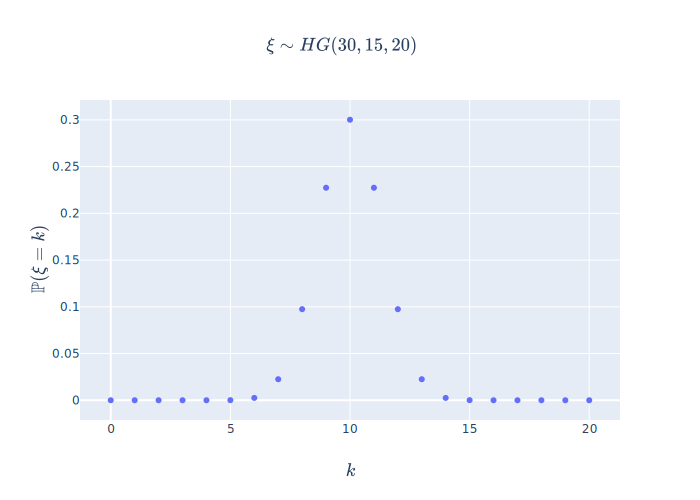
\includegraphics{../assets/hg_hist.svg}
\caption{Гистограмма вероятностей гипергеометрического распределения}
\end{figure}

\hypertarget{ux444ux443ux43dux43aux446ux438ux44f-ux440ux430ux441ux43fux440ux435ux434ux435ux43bux435ux43dux438ux44f}{%
\paragraph{Функция
распределения}\label{ux444ux443ux43dux43aux446ux438ux44f-ux440ux430ux441ux43fux440ux435ux434ux435ux43bux435ux43dux438ux44f}}

По определению, функция распределения
\(F_\xi(k) = \mathbb{P}\left(\, \xi < k \,\right)\). Для дискретной
случайной величины событие
\(\{\xi < k\} = \bigcup\limits_{i=0}^{k-1}\{\xi=i\}\). Каждое из событий
\(\{\xi=i\}\; \forall i \in \overline{0, k-1}\) являются попарно
несовместными. То есть \(\forall i,j \in \overline{0, k-1}: i \neq j\)
выполняется \(\{\xi=i\}\cap\{\xi=j\}=\emptyset\). Из этого следует, что
\[\mathbb{P}\left(\, \xi < k \,\right) = \sum_{i=0}^{k-1}\mathbb{P}\left(\, \xi = i \,\right)\]
Подставим \ref{eq:hg_def} в это выражение и получим: \[F_\xi(k)
= \sum_{i=0}^{k-1}\mathbb{P}\left(\, \xi = i \,\right)
= \sum_{i=0}^{k-1}\frac{\binom{m}{i}\binom{N-m}{n-i}}{\binom{N}{n}}\]

Построим график этой функции, учитывая, что аргументом \(k\) должно быть
натуральное число, не превосходящее \(n\):

\begin{lstlisting}[language=Python, numbers=left, firstnumber=40]
n_dist_fig = go.Figure(
    data=(go.Scatter(
        x=list(n_data_x),
        y=list(map(eta.p, n_data_x)),
    ),),
    layout=go.Layout(
        title=go.layout.Title(
            text=r'$\eta \sim ' + str(eta) + '$',
            x=.5,
        ),
        yaxis=go.layout.YAxis(
            title=go.layout.yaxis.Title(
                text=r'$\mathbb{P}(\eta<x)$',
            ),
        ),
        xaxis=go.layout.XAxis(
            title=go.layout.xaxis.Title(
                text=r'$x$',
            ),
        ),
    ),
)
plotly.offline.iplot(n_dist_fig)
\end{lstlisting}

График будет следующим:

\begin{figure}
\centering
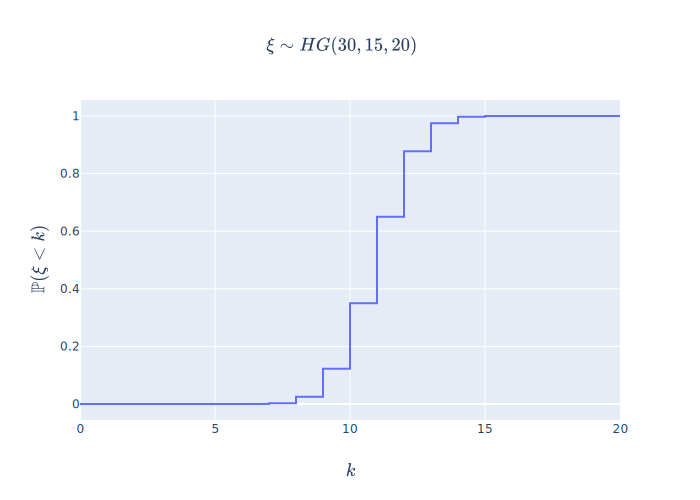
\includegraphics{../assets/hg_dist.svg}
\caption{Функция распределения гипергеометрического распределния}
\end{figure}

\hypertarget{ux43dux43eux440ux43cux430ux43bux44cux43dux43eux435-ux440ux430ux441ux43fux440ux435ux434ux435ux43bux435ux43dux438ux435}{%
\subsubsection{Нормальное
распределение}\label{ux43dux43eux440ux43cux430ux43bux44cux43dux43eux435-ux440ux430ux441ux43fux440ux435ux434ux435ux43bux435ux43dux438ux435}}

Нормальное распределение - непрерывное распределение, описывающее
поведение величины отклонения измеряемого значения \(x\) от истинного
значения \(\mu\) (которое является математическим ожиданием) и в рамках
некоторого разброса \(\sigma\) (среднеквадратичного отклонения). Запишем
это формально:
\begin{equation}\left\{ \eta \sim N(\mu, \sigma^2) \right\}
\iff
\left\{\begin{gathered}
    F_\eta(x) = \mathbb{P}\left(\, \eta < x \,\right) = \int_{-\infty}^{x} f_\eta(x)dx,\\
    \text{где } f_\eta(x) = \frac{1}{\sigma\sqrt{2\pi}}e^{-\frac{(x-\mu)^2}{2\sigma^2}} \text{– плотность вероятности}
\end{gathered}\right\}\label{eq:norm_def}\end{equation}

\hypertarget{ux43cux430ux442ux435ux43cux430ux442ux438ux447ux435ux441ux43aux43eux435-ux43eux436ux438ux434ux430ux43dux438ux435-1}{%
\paragraph{Математическое
ожидание}\label{ux43cux430ux442ux435ux43cux430ux442ux438ux447ux435ux441ux43aux43eux435-ux43eux436ux438ux434ux430ux43dux438ux435-1}}

Найдем математическое ожидание \(\eta \sim N(\mu, \sigma^2)\):
\[\begin{aligned}
    \mathbb{E}\left[\, \eta \,\right] &= \int_{-\infty}^{+\infty} x \cdot f_\eta(x)dx =\\
                  &= \int_{-\infty}^{+\infty} xe^{-\frac{(x-\mu)^2}{2\sigma^2}}dx =\\
                  &= \frac{1}{\sigma\sqrt{2\pi}} \int_{-\infty}^{+\infty} xe^{-\frac{(x-\mu)^2}{2\sigma^2}}dx
\end{aligned}\] Сделаем замену \(t = \frac{x-\mu}{\sqrt{2}\sigma}\):
\[\begin{aligned}
    \mathbb{E}\left[\, \eta \,\right] &= \frac{1}{\sigma\sqrt{2\pi}} \int_{-\infty}^{+\infty}(\sigma\sqrt{2}t + \mu)
                    e^{-t^2} d\left(\frac{x-\mu}{\sqrt{2}\sigma}\right) =\\
                  &= \frac{\sigma\sqrt{2}}{\sqrt{\pi}}\int_{-\infty}^{+\infty}te^{-t^2}dt
                    + \frac{\mu}{\sqrt{\pi}}\int_{-\infty}^{+\infty}e^{-t^2}dt =\\
                  &= \frac{\sigma\sqrt{2}}{\sqrt{\pi}}\left(\int_{-\infty}^{0}te^{-t^2}dt
                    - \int_{-\infty}^{0}te^{-t^2}dt\right) + \frac{\mu}{\sqrt{\pi}}\int_{-\infty}^{+\infty}e^{-t^2}dt =\\
                  &= \frac{\mu}{\sqrt{\pi}}\int_{-\infty}^{+\infty}e^{-t^2}dt
\end{aligned}\] Заметим, что получившееся выражение содержит интеграл,
который может быть сведен к интегралу
\href{https://ru.wikipedia.org/wiki/Гауссов_интеграл}{Эйлера-Пуассона}:
\[\int_{-\infty}^{+\infty}e^{-t^2}dt = 2\int_{0}^{+\infty}e^{-t^2}dt = \sqrt{\pi}\]
Таким образом, \begin{equation}\boxed{
    \mathbb{E}\left[\, \eta \,\right] = \mu
}\label{eq:n_expected}\end{equation}

\hypertarget{ux434ux438ux441ux43fux435ux440ux441ux438ux44f-1}{%
\paragraph{Дисперсия}\label{ux434ux438ux441ux43fux435ux440ux441ux438ux44f-1}}

Подставим \ref{eq:n_expected} в определение дисперсии
\ref{eq:variance_def}: \[\begin{aligned}
    \mathrm{Var}\left[\, \eta \,\right] &= \mathbb{E}\left[\, (\eta - \mu)^2 \,\right] =\\
               &= \int_{-\infty}^{+\infty} (x-\mu)^2 \cdot f_{\eta}(x)dx =\\
               &= \int_{-\infty}^{+\infty}(x-\mu)^2 \frac{1}{\sigma\sqrt{2\pi}}e^{-\frac{(x-\mu)^2}{2\sigma^2}}dx =\\
               &= \frac{1}{\sigma\sqrt{2\pi}}\int_{-\infty}^{+\infty}(x-\mu)^2 e^{-\frac{(x-\mu)^2}{2\sigma^2}}dx
\end{aligned}\] Сделаем ту же замену переменной
\(t = \frac{x-\mu}{\sqrt{2}\sigma}\), тогда \(x = t\sqrt{2}\sigma+\mu\)
и: \[\begin{aligned}
    \mathrm{Var}\left[\, \eta \,\right] &= \frac{1}{\sigma\sqrt{2\pi}}
                \int_{-\infty}^{+\infty}(\sqrt{2}\sigma)^2 t^2 e^{-t^2}d(t\sqrt{2}\sigma+\mu) =\\
               &= \frac{2\sigma^2}{\sqrt{\pi}}\int_{-\infty}^{+\infty}t^2 e^{-t^2}dt
\end{aligned}\] Проинтегрируем по частям: \[\begin{aligned}
    \mathrm{Var}\left[\, \eta \,\right] &= \frac{\sigma^2}{\sqrt{\pi}}\int_{-\infty}^{+\infty}t 2t e^{-t^2} dt =\\
               &= \frac{\sigma^2}{\sqrt{\pi}}\left(\left. -t e^{-t^2} \right|_{-\infty}^{+\infty}
                 + \int_{-\infty}^{+\infty}e^{-t^2}dt\right)
\end{aligned}\] Здесь снова появляется интеграл
\href{https://ru.wikipedia.org/wiki/Гауссов_интеграл}{Эйлера-Пуассона}
и, в итоге, получаем: \[\boxed{
    \mathrm{Var}\left[\, \eta \,\right] = \sigma^2
}\] То есть, \(\sigma\) является среднеквадратичным отклонением.

\hypertarget{ux43fux440ux43eux438ux437ux432ux43eux434ux44fux449ux430ux44f-ux444ux443ux43dux43aux446ux438ux44f-ux43cux43eux43cux435ux43dux442ux43eux432-1}{%
\paragraph{Производящая функция
моментов}\label{ux43fux440ux43eux438ux437ux432ux43eux434ux44fux449ux430ux44f-ux444ux443ux43dux43aux446ux438ux44f-ux43cux43eux43cux435ux43dux442ux43eux432-1}}

Производящая функция моментов для \(\eta \sim N(\mu, \sigma^2)\) имеет
вид: \[M_\eta(t) = \exp\left(\mu t + \frac{\sigma^2 t^2}{2}\right)\]

\hypertarget{ux445ux430ux440ux430ux43aux442ux435ux440ux438ux441ux442ux438ux447ux435ux441ux43aux430ux44f-ux444ux443ux43dux43aux446ux438ux44f-1}{%
\paragraph{Характеристическая
функция}\label{ux445ux430ux440ux430ux43aux442ux435ux440ux438ux441ux442ux438ux447ux435ux441ux43aux430ux44f-ux444ux443ux43dux43aux446ux438ux44f-1}}

Характеристическая функция для \(\eta \sim N(\mu, \sigma^2)\) имеет вид:
\[\varphi_\eta(t) = \exp\left(\mu it + \frac{\sigma^2 t^2}{2}\right)\]

\hypertarget{ux43fux43bux43eux442ux43dux43eux441ux442ux44c-ux432ux435ux440ux43eux44fux442ux43dux43eux441ux442ux438}{%
\paragraph{Плотность
вероятности}\label{ux43fux43bux43eux442ux43dux43eux441ux442ux44c-ux432ux435ux440ux43eux44fux442ux43dux43eux441ux442ux438}}

Определим класс нормального распределения \passthrough{\lstinline!N!},
который будет содержать в себе информацию о параметрах \(\mu\) и
\(\sigma\) и предоставлять следующие методы:

\begin{itemize}
\tightlist
\item
  \passthrough{\lstinline!f(x)!} - возвращает значение плотности в точке
  \passthrough{\lstinline!x!}
\item
  \passthrough{\lstinline!p(k)!} - возвращает
  \(\mathbb{P}\left(\, \eta < x \,\right) = \int_{-\infty}^x f_\eta(x)dx\)
\end{itemize}

\begin{lstlisting}[language=Python, numbers=left, firstnumber=1]
class N(object):
    def __init__(self, mu: float, sigma: float):
        self.mu = mu
        self.sigma = sigma
    def f(self, x: float) -> float:
        return np.exp(-((x-self.mu)**2)/(2*self.sigma**2))/(self.sigma*(2*np.pi)**.5)
    def p(self, x: float) -> float:
        return sp.integrate.quad(self.f, -np.inf, x)[0]
    def __str__(self):
        return f'N({self.mu}, {self.sigma}^2)'
\end{lstlisting}

Далее создадим объект случайной величины \(\xi \sim HG(30, 15, 20)\):

\begin{lstlisting}[language=Python, numbers=left, firstnumber=11]
eta = N(0, 1)
\end{lstlisting}

Следующим шагом, руководствуясь
\href{https://ru.wikipedia.org/wiki/Среднеквадратическое_отклонение\#Правило_трёх_сигм}{правилом
трех сигм}определим интервал \((-3\sigma, 3\sigma)\):

\begin{lstlisting}[language=Python, numbers=left, firstnumber=12]
n_data_x = np.linspace(-3*eta.sigma, 3*eta.sigma, 100)
\end{lstlisting}

И, наконец, построим плотность, используя метод
\passthrough{\lstinline!N.f!} нашего класса:

\begin{lstlisting}[language=Python, numbers=left, firstnumber=13]
n_dens_fig = go.Figure(
    data=(go.Scatter(
        x=list(n_data_x),
        y=list(map(eta.f, n_data_x)),
    ),),
    layout=go.Layout(
        title=go.layout.Title(
            text=r'$\eta \sim ' + str(eta) + '$',
            x=.5,
        ),
        yaxis=go.layout.YAxis(
            title=go.layout.yaxis.Title(
                text=r'$f_\eta(x)$',
            ),
        ),
        xaxis=go.layout.XAxis(
            title=go.layout.xaxis.Title(
                text=r'$x$',
            ),
        ),
    ),
)
plotly.offline.iplot(n_dens_fig)
\end{lstlisting}

Получившийся график имеет следующий вид:

\begin{figure}
\centering
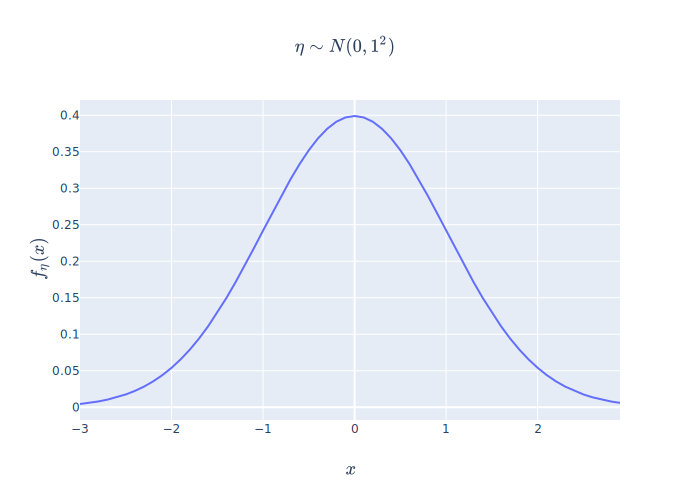
\includegraphics{../assets/n_density.svg}
\caption{Плотность нормального распределения}
\end{figure}

\hypertarget{ux444ux443ux43dux43aux446ux438ux44f-ux440ux430ux441ux43fux440ux435ux434ux435ux43bux435ux43dux438ux44f-1}{%
\paragraph{Функция
распределения}\label{ux444ux443ux43dux43aux446ux438ux44f-ux440ux430ux441ux43fux440ux435ux434ux435ux43bux435ux43dux438ux44f-1}}

Для построения функции распределения, будем использовать метод
\passthrough{\lstinline!N.p!}:

\begin{lstlisting}[language=Python, numbers=left, firstnumber=37]
n_dist_fig = go.Figure(
    data=(
        go.Scatter(
            x=list(n_data_x),
            y=list(map(eta.p, n_data_x)),
        ),
    ),
    layout=go.Layout(
        title=go.layout.Title(
            text=r'$\eta \sim ' + str(eta) + '$',
            x=.5,
        ),
        yaxis=go.layout.YAxis(
            title=go.layout.yaxis.Title(
                text=r'$\mathbb{P}(\eta<x)$',
            ),
        ),
        xaxis=go.layout.XAxis(
            title=go.layout.xaxis.Title(
                text=r'$x$',
            ),
        ),
    ),
)
plotly.offline.iplot(n_dist_fig)
\end{lstlisting}

Функция распределения имеет вид:

\begin{figure}
\centering
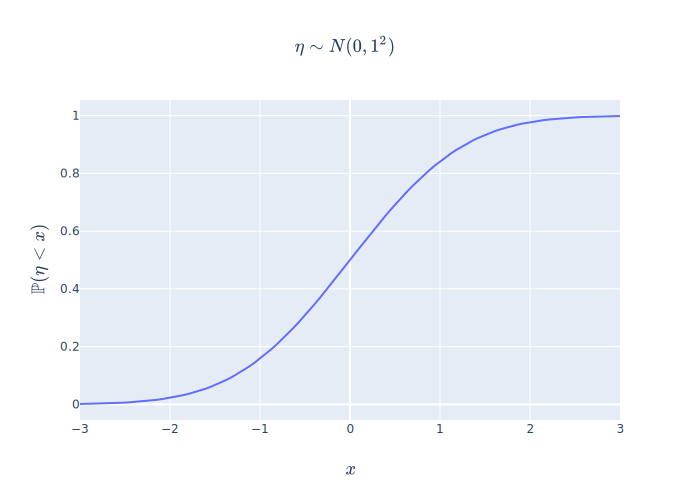
\includegraphics{../assets/n_distribution.svg}
\caption{Функция распределения нормального распределения}
\end{figure}

\hypertarget{ux43fux440ux438ux43cux435ux440ux44b-ux441ux43eux431ux44bux442ux438ux439-ux438-ux438ux43dux442ux435ux440ux43fux440ux435ux442ux430ux446ux438ux438}{%
\subsection{Примеры событий и
интерпретации}\label{ux43fux440ux438ux43cux435ux440ux44b-ux441ux43eux431ux44bux442ux438ux439-ux438-ux438ux43dux442ux435ux440ux43fux440ux435ux442ux430ux446ux438ux438}}

\hypertarget{ux433ux438ux43fux435ux440ux433ux435ux43eux43cux435ux442ux440ux438ux447ux435ux441ux43aux43eux435-ux440ux430ux441ux43fux440ux435ux434ux435ux43bux435ux43dux438ux435-1}{%
\subsubsection{Гипергеометрическое
распределение}\label{ux433ux438ux43fux435ux440ux433ux435ux43eux43cux435ux442ux440ux438ux447ux435ux441ux43aux43eux435-ux440ux430ux441ux43fux440ux435ux434ux435ux43bux435ux43dux438ux435-1}}

\hypertarget{ux442ux438ux43fux438ux447ux43dux430ux44f-ux438ux43dux442ux435ux440ux43fux440ux435ux442ux430ux446ux438ux44f}{%
\paragraph{Типичная
интерпретация}\label{ux442ux438ux43fux438ux447ux43dux430ux44f-ux438ux43dux442ux435ux440ux43fux440ux435ux442ux430ux446ux438ux44f}}

Типичной интерпретацией гипергеометрического распределения является
выборка без возвращения из множества элементов, некоторые из которых
являются помеченными. Представим, что в нашем распоряжении имеется
корзина, наполненная шарами двух цветов: черные и белые. Причём всего в
корзине находится \(N\) шаров, \(m\) из которых -- белые. Шары в корзине
тщательно перемешиваются, чтобы каждый из них мог быть вытащен с
одинаковой вероятностью \(\frac{1}{N}\). Далее случайно вытаскиваются
\(n\) шаров без возвращения. Гипергеометрическое распределение описывает
вероятность того, что среди вытащенных шаров ровно \(k\) окажутся
белыми.

Действительно, всего существует \(\binom{N}{n}\) выборок размера \(n\),
\(\binom{m}{k}\) способов выбрать \(k\) помеченных объектов (белых
шаров), и \(\binom{N-m}{n-k}\) способов заполнить оставшиеся \(n-k\)
\emph{слотов} непомеченными объектами (черными шарами). Таким образом,
вероятность того, что среди \(n\) вытащенных объектов окажется ровно
\(k\) помеченных, будет равна
\(\frac{\binom{m}{k}\binom{N-m}{n-k}}{\binom{N}{n}}\).

\hypertarget{ux438ux437ux432ux435ux441ux442ux43dux44bux435-ux441ux43eux43eux442ux43dux43eux448ux435ux43dux438ux44f-ux43cux435ux436ux434ux443-ux440ux430ux441ux43fux440ux435ux434ux435ux43bux435ux43dux438ux44fux43cux438}{%
\paragraph{Известные соотношения между
распределениями}\label{ux438ux437ux432ux435ux441ux442ux43dux44bux435-ux441ux43eux43eux442ux43dux43eux448ux435ux43dux438ux44f-ux43cux435ux436ux434ux443-ux440ux430ux441ux43fux440ux435ux434ux435ux43bux435ux43dux438ux44fux43cux438}}

\begin{itemize}
\tightlist
\item
  Если зафиксировать размер выборки и количество помеченных элементов, а
  мощность множества, из которого ведется выборка, устремить к
  бесконечности, то гипергеометрическое распределение будет сходиться к
  биномиальному:
  \[HG(N, m, n) \underset{N\to\infty}{\longrightarrow} Bi\left(n, \frac{m}{N}\right)\]
\end{itemize}

\hypertarget{ux43dux43eux440ux43cux430ux43bux44cux43dux43eux435-ux440ux430ux441ux43fux440ux435ux434ux435ux43bux435ux43dux438ux435-1}{%
\subsubsection{Нормальное
распределение}\label{ux43dux43eux440ux43cux430ux43bux44cux43dux43eux435-ux440ux430ux441ux43fux440ux435ux434ux435ux43bux435ux43dux438ux435-1}}

\hypertarget{ux442ux438ux43fux438ux447ux43dux430ux44f-ux438ux43dux442ux435ux440ux43fux440ux435ux442ux430ux446ux438ux44f-1}{%
\paragraph{Типичная
интерпретация}\label{ux442ux438ux43fux438ux447ux43dux430ux44f-ux438ux43dux442ux435ux440ux43fux440ux435ux442ux430ux446ux438ux44f-1}}

Нормальное распределение описывает нормированную случайную величину,
которая является суммой многих случайных слабо взаимосвязанных величин,
каждая из которых вносит малый вклад относительно общей суммы. Это
вытекает из
\href{https://ru.wikipedia.org/wiki/Центральная_предельная_теорема}{центральной
предельной теоремы}.

\hypertarget{ux438ux437ux432ux435ux441ux442ux43dux44bux435-ux441ux43eux43eux442ux43dux43eux448ux435ux43dux438ux44f-ux43cux435ux436ux434ux443-ux440ux430ux441ux43fux440ux435ux434ux435ux43bux435ux43dux438ux44fux43cux438-1}{%
\paragraph{Известные соотношения между
распределениями}\label{ux438ux437ux432ux435ux441ux442ux43dux44bux435-ux441ux43eux43eux442ux43dux43eux448ux435ux43dux438ux44f-ux43cux435ux436ux434ux443-ux440ux430ux441ux43fux440ux435ux434ux435ux43bux435ux43dux438ux44fux43cux438-1}}

\begin{itemize}
\item
  Сумма двух независимых случайных величин, имеющих нормальное
  распределение, имеет
  \href{https://ru.wikipedia.org/wiki/Распределение_Коши}{распределение
  Коши}: \[\begin{aligned}
  \xi\ &\sim\ N(\mu_1, {\sigma_1}^2)\\
  \eta\ &\sim\ N(\mu_2, {\sigma_2}^2)\\
  \xi+\eta\ &\sim\ C(\mu_1 + \mu_2, \sqrt{{\sigma_1}^2 + {\sigma_2}^2})
  \end{aligned}\] 
\item
  Сумма квадратов \(k\) независимых стандартных нормальных случайных
  величин имеет
  \href{https://ru.wikipedia.org/wiki/Распределение_хи-квадрат}{распределение
  \(\chi^2\)} c \(k\) степенями свободы: \[\begin{aligned}
  \forall i \in \overline{1, k}\quad \xi_i\ &\sim\ N(0, 1)\\
  \sum_{i=1}^k \xi_i &\sim \chi^2(k)
  \end{aligned}\]
\item
  Натуральный логарифм
  \href{https://ru.wikipedia.org/wiki/Логнормальное_распределение}{логнормального
  распределения} имеет нормальное распределение: \[\begin{aligned}
  \xi &\sim LogN(\mu,\sigma^2)\\
  \ln\xi &\sim N(\mu,\sigma^2)
  \end{aligned}\]
\end{itemize}

\hypertarget{ux441ux43fux43eux441ux43eux431ux44b-ux43cux43eux434ux435ux43bux438ux440ux43eux432ux430ux43dux438ux44f-ux441ux43bux443ux447ux430ux439ux43dux44bux445-ux432ux435ux43bux438ux447ux438ux43d}{%
\subsection{Способы моделирования случайных
величин}\label{ux441ux43fux43eux441ux43eux431ux44b-ux43cux43eux434ux435ux43bux438ux440ux43eux432ux430ux43dux438ux44f-ux441ux43bux443ux447ux430ux439ux43dux44bux445-ux432ux435ux43bux438ux447ux438ux43d}}

Для моделирования выбранных случайных величин, будем использовать
библиотеку \href{https://www.scipy.org}{SciPy}.

\hypertarget{ux433ux438ux43fux435ux440ux433ux435ux43eux43cux435ux442ux440ux438ux447ux435ux441ux43aux43eux435-ux440ux430ux441ux43fux440ux435ux434ux435ux43bux435ux43dux438ux435-2}{%
\subsubsection{Гипергеометрическое
распределение}\label{ux433ux438ux43fux435ux440ux433ux435ux43eux43cux435ux442ux440ux438ux447ux435ux441ux43aux43eux435-ux440ux430ux441ux43fux440ux435ux434ux435ux43bux435ux43dux438ux435-2}}

Для моделирования гипергеометрического распределения будем использовать
класс
\href{https://docs.scipy.org/doc/scipy/reference/generated/scipy.stats.hypergeom.html}{\passthrough{\lstinline!scipy.stats.hypergeom!}}:

\begin{lstlisting}[language=Python]
hg = sp.stats.hypergeom(xi.N,xi.m,xi.n)
\end{lstlisting}

Проверим, что \passthrough{\lstinline!hg.pmf!} возвращает правильные
значения для вероятности. Для этого построим с помощью этой функции
гистограмму и наложим ее на ту, которую мы получали ранее:

\begin{lstlisting}[language=Python, numbers=left]
hg_model_fig = go.Figure(
    data=(
        go.Scatter(
            name=f'model',
            x=list(hg_data_x),
            y=hg.pmf(hg_data_x),
            mode='markers',
            marker_size=10,
        ),
        hg_hist_plot,
    ),
    layout=go.Layout(
        title=go.layout.Title(
            text=r'$\xi \sim ' + str(xi) + '$',
            x=.5,
        ),
        yaxis=go.layout.YAxis(title=go.layout.yaxis.Title(
            text=r'$\mathbb{P}(\xi=k)$',
        )),
        xaxis=go.layout.XAxis(title=go.layout.xaxis.Title(
            text=r'$k$',
        )),
    ),
)
plotly.offline.iplot(hg_model_fig)
\end{lstlisting}

График получится следующий:

\begin{figure}
\centering
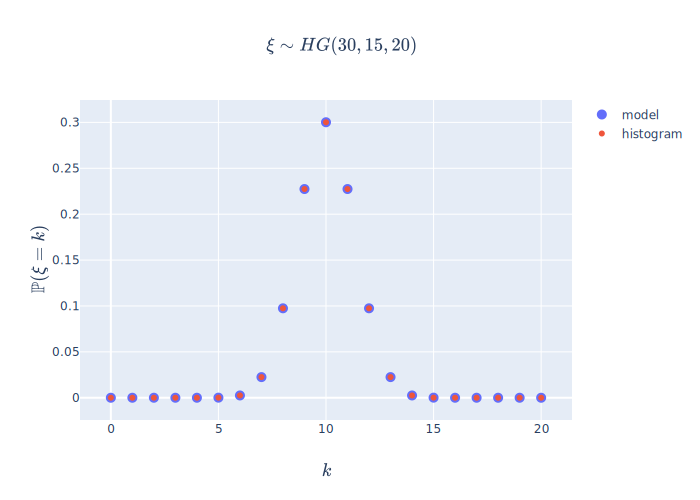
\includegraphics{../assets/hg_model_fig.svg}
\caption{Проверка функции генерации выборки из гипергеометрического
распределения с помощью SciPy}
\end{figure}

\hypertarget{ux43dux43eux440ux43cux430ux43bux44cux43dux43eux435-ux440ux430ux441ux43fux440ux435ux434ux435ux43bux435ux43dux438ux435-2}{%
\subsubsection{Нормальное
распределение}\label{ux43dux43eux440ux43cux430ux43bux44cux43dux43eux435-ux440ux430ux441ux43fux440ux435ux434ux435ux43bux435ux43dux438ux435-2}}

Для моделирования нормального распределения будем использовать класс
\href{https://docs.scipy.org/doc/scipy/reference/generated/scipy.stats.hypergeom.html}{\passthrough{\lstinline!scipy.stats.norm!}}:

\begin{lstlisting}[language=Python]
n = sp.stats.norm(eta.mu,eta.sigma)
\end{lstlisting}

Проверим, что \passthrough{\lstinline!n.pdf!} возвращает правильные
значения для вероятности. Для этого построим с помощью этой функции
плотность и наложим ее на ту, которую мы получали ранее:

\begin{lstlisting}[language=Python, numbers=left]
n_model_fig = go.Figure(
    data=(
        go.Scatter(
            name=f'model',
            x=list(n_data_x),
            y=n.pdf(n_data_x),
            line_width=8,
        ),
        n_dens_plot,
    ),
    layout=go.Layout(
        title=go.layout.Title(
            text=r'$\eta \sim ' + str(eta) + '$',
            x=.5,
        ),
        yaxis=go.layout.YAxis(title=go.layout.yaxis.Title(
            text=r'$f_\eta(x)$',
        )),
        xaxis=go.layout.XAxis(title=go.layout.xaxis.Title(
            text=r'$x$',
        )),
    ),
)
plotly.offline.iplot(n_model_fig)
\end{lstlisting}

График получится следующий:

\begin{figure}
\centering
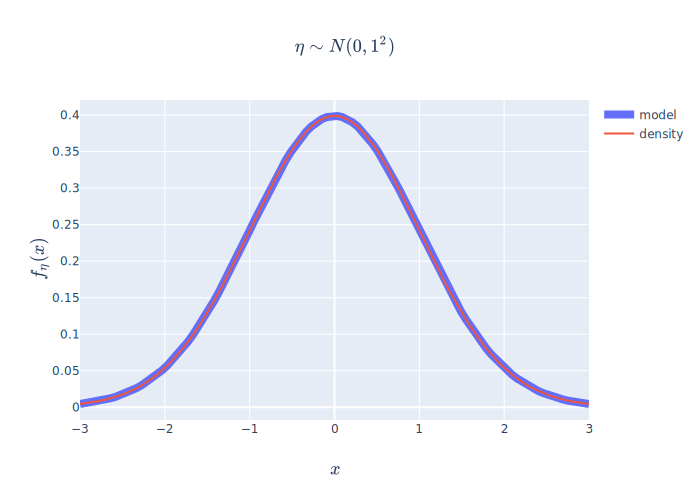
\includegraphics{../assets/n_model_fig.svg}
\caption{Проверка функции генерации выборки из нормального распределения
с помощью SciPy}
\end{figure}

\end{document}
